\documentclass[twoside]{book}

% Packages required by doxygen
\usepackage{fixltx2e}
\usepackage{calc}
\usepackage{doxygen}
\usepackage[export]{adjustbox} % also loads graphicx
\usepackage{graphicx}
\usepackage[utf8]{inputenc}
\usepackage{makeidx}
\usepackage{multicol}
\usepackage{multirow}
\PassOptionsToPackage{warn}{textcomp}
\usepackage{textcomp}
\usepackage[nointegrals]{wasysym}
\usepackage[table]{xcolor}

% Font selection
\usepackage[T1]{fontenc}
\usepackage[scaled=.90]{helvet}
\usepackage{courier}
\usepackage{amssymb}
\usepackage{sectsty}
\renewcommand{\familydefault}{\sfdefault}
\allsectionsfont{%
  \fontseries{bc}\selectfont%
  \color{darkgray}%
}
\renewcommand{\DoxyLabelFont}{%
  \fontseries{bc}\selectfont%
  \color{darkgray}%
}
\newcommand{\+}{\discretionary{\mbox{\scriptsize$\hookleftarrow$}}{}{}}

% Page & text layout
\usepackage{geometry}
\geometry{%
  a4paper,%
  top=2.5cm,%
  bottom=2.5cm,%
  left=2.5cm,%
  right=2.5cm%
}
\tolerance=750
\hfuzz=15pt
\hbadness=750
\setlength{\emergencystretch}{15pt}
\setlength{\parindent}{0cm}
\setlength{\parskip}{3ex plus 2ex minus 2ex}
\makeatletter
\renewcommand{\paragraph}{%
  \@startsection{paragraph}{4}{0ex}{-1.0ex}{1.0ex}{%
    \normalfont\normalsize\bfseries\SS@parafont%
  }%
}
\renewcommand{\subparagraph}{%
  \@startsection{subparagraph}{5}{0ex}{-1.0ex}{1.0ex}{%
    \normalfont\normalsize\bfseries\SS@subparafont%
  }%
}
\makeatother

% Headers & footers
\usepackage{fancyhdr}
\pagestyle{fancyplain}
\fancyhead[LE]{\fancyplain{}{\bfseries\thepage}}
\fancyhead[CE]{\fancyplain{}{}}
\fancyhead[RE]{\fancyplain{}{\bfseries\leftmark}}
\fancyhead[LO]{\fancyplain{}{\bfseries\rightmark}}
\fancyhead[CO]{\fancyplain{}{}}
\fancyhead[RO]{\fancyplain{}{\bfseries\thepage}}
\fancyfoot[LE]{\fancyplain{}{}}
\fancyfoot[CE]{\fancyplain{}{}}
\fancyfoot[RE]{\fancyplain{}{\bfseries\scriptsize Generated by Doxygen }}
\fancyfoot[LO]{\fancyplain{}{\bfseries\scriptsize Generated by Doxygen }}
\fancyfoot[CO]{\fancyplain{}{}}
\fancyfoot[RO]{\fancyplain{}{}}
\renewcommand{\footrulewidth}{0.4pt}
\renewcommand{\chaptermark}[1]{%
  \markboth{#1}{}%
}
\renewcommand{\sectionmark}[1]{%
  \markright{\thesection\ #1}%
}

% Indices & bibliography
\usepackage{natbib}
\usepackage[titles]{tocloft}
\setcounter{tocdepth}{3}
\setcounter{secnumdepth}{5}
\makeindex

% Hyperlinks (required, but should be loaded last)
\usepackage{ifpdf}
\ifpdf
  \usepackage[pdftex,pagebackref=true]{hyperref}
\else
  \usepackage[ps2pdf,pagebackref=true]{hyperref}
\fi
\hypersetup{%
  colorlinks=true,%
  linkcolor=blue,%
  citecolor=blue,%
  unicode%
}

% Custom commands
\newcommand{\clearemptydoublepage}{%
  \newpage{\pagestyle{empty}\cleardoublepage}%
}

\usepackage{caption}
\captionsetup{labelsep=space,justification=centering,font={bf},singlelinecheck=off,skip=4pt,position=top}

%===== C O N T E N T S =====

\begin{document}

% Titlepage & ToC
\hypersetup{pageanchor=false,
             bookmarksnumbered=true,
             pdfencoding=unicode
            }
\pagenumbering{roman}
\begin{titlepage}
\vspace*{7cm}
\begin{center}%
{\Large My Project }\\
\vspace*{1cm}
{\large Generated by Doxygen 1.8.11}\\
\end{center}
\end{titlepage}
\clearemptydoublepage
\tableofcontents
\clearemptydoublepage
\pagenumbering{arabic}
\hypersetup{pageanchor=true}

%--- Begin generated contents ---
\chapter{Hierarchical Index}
\section{Class Hierarchy}
This inheritance list is sorted roughly, but not completely, alphabetically\+:\begin{DoxyCompactList}
\item \contentsline{section}{Fruit}{\pageref{classFruit}}{}
\begin{DoxyCompactList}
\item \contentsline{section}{Apple}{\pageref{classApple}}{}
\item \contentsline{section}{Grape}{\pageref{classGrape}}{}
\item \contentsline{section}{Orange}{\pageref{classOrange}}{}
\end{DoxyCompactList}
\item \contentsline{section}{List}{\pageref{classList}}{}
\item \contentsline{section}{List\+:\+:Node}{\pageref{structList_1_1Node}}{}
\end{DoxyCompactList}

\chapter{Class Index}
\section{Class List}
Here are the classes, structs, unions and interfaces with brief descriptions\+:\begin{DoxyCompactList}
\item\contentsline{section}{\hyperlink{structnode}{node} }{\pageref{structnode}}{}
\item\contentsline{section}{\hyperlink{structnode1}{node1} }{\pageref{structnode1}}{}
\item\contentsline{section}{\hyperlink{structnode__info}{node\+\_\+info} }{\pageref{structnode__info}}{}
\end{DoxyCompactList}

\chapter{File Index}
\section{File List}
Here is a list of all files with brief descriptions\+:\begin{DoxyCompactList}
\item\contentsline{section}{\hyperlink{Lab1_8c}{Lab1.\+c} }{\pageref{Lab1_8c}}{}
\end{DoxyCompactList}

\chapter{Class Documentation}
\hypertarget{classCurrentConditionBoard}{}\section{Current\+Condition\+Board Class Reference}
\label{classCurrentConditionBoard}\index{Current\+Condition\+Board@{Current\+Condition\+Board}}


Inheritance diagram for Current\+Condition\+Board\+:
\nopagebreak
\begin{figure}[H]
\begin{center}
\leavevmode
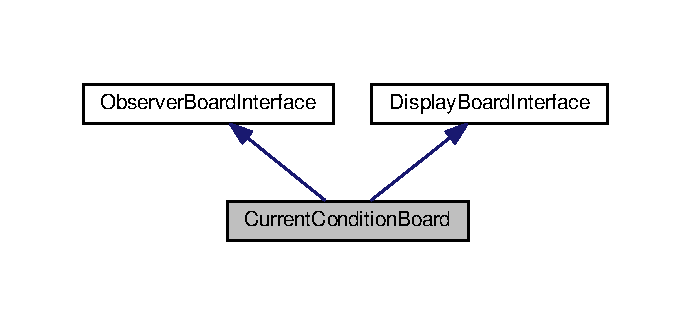
\includegraphics[width=332pt]{classCurrentConditionBoard__inherit__graph}
\end{center}
\end{figure}


Collaboration diagram for Current\+Condition\+Board\+:
\nopagebreak
\begin{figure}[H]
\begin{center}
\leavevmode
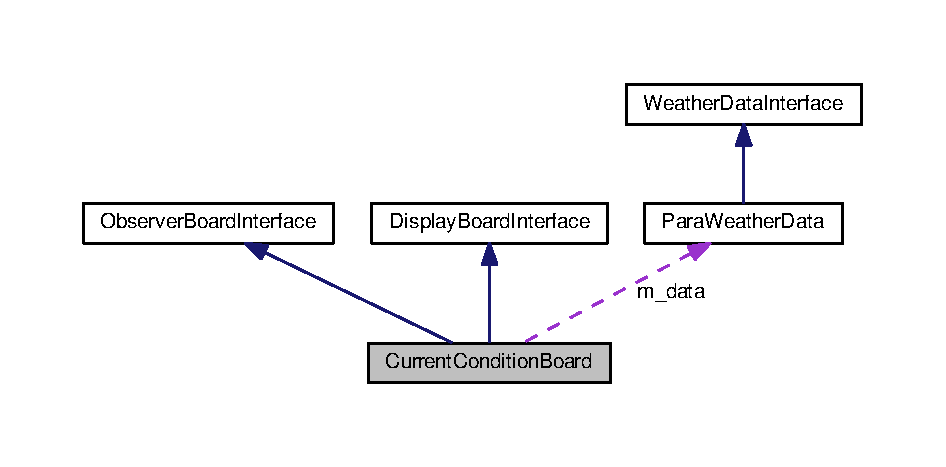
\includegraphics[width=350pt]{classCurrentConditionBoard__coll__graph}
\end{center}
\end{figure}
\subsection*{Public Member Functions}
\begin{DoxyCompactItemize}
\item 
\hyperlink{classCurrentConditionBoard_ae25ee112ee83575673b3e4f8448f1da7}{Current\+Condition\+Board} (\hyperlink{classParaWeatherData}{Para\+Weather\+Data} \&a)
\item 
void \hyperlink{classCurrentConditionBoard_a5cd2077415a0e7019c15bc0f28cfb7fe}{show} ()
\item 
void \hyperlink{classCurrentConditionBoard_a3d7bea56331de46f30db9e93f8f2c7d3}{update} (float h, float t, float p)
\end{DoxyCompactItemize}
\subsection*{Private Attributes}
\begin{DoxyCompactItemize}
\item 
float \hyperlink{classCurrentConditionBoard_a0fb59476afc70b786750c2b0e87ced7a}{m\+\_\+h}
\item 
float \hyperlink{classCurrentConditionBoard_a443f62d33750e33fc12554c084b57c7f}{m\+\_\+t}
\item 
float \hyperlink{classCurrentConditionBoard_ab36a854fdba3f5b6fc30624bdefa18f3}{m\+\_\+p}
\item 
\hyperlink{classParaWeatherData}{Para\+Weather\+Data} \& \hyperlink{classCurrentConditionBoard_abb74e202395a04791f3526d2bab123dd}{m\+\_\+data}
\end{DoxyCompactItemize}


\subsection{Constructor \& Destructor Documentation}
\index{Current\+Condition\+Board@{Current\+Condition\+Board}!Current\+Condition\+Board@{Current\+Condition\+Board}}
\index{Current\+Condition\+Board@{Current\+Condition\+Board}!Current\+Condition\+Board@{Current\+Condition\+Board}}
\subsubsection[{\texorpdfstring{Current\+Condition\+Board(\+Para\+Weather\+Data \&a)}{CurrentConditionBoard(ParaWeatherData &a)}}]{\setlength{\rightskip}{0pt plus 5cm}Current\+Condition\+Board\+::\+Current\+Condition\+Board (
\begin{DoxyParamCaption}
\item[{{\bf Para\+Weather\+Data} \&}]{a}
\end{DoxyParamCaption}
)\hspace{0.3cm}{\ttfamily [inline]}}\hypertarget{classCurrentConditionBoard_ae25ee112ee83575673b3e4f8448f1da7}{}\label{classCurrentConditionBoard_ae25ee112ee83575673b3e4f8448f1da7}

\begin{DoxyCode}
73                                              :\hyperlink{classCurrentConditionBoard_abb74e202395a04791f3526d2bab123dd}{m\_data}(a)
74     \{
75         \hyperlink{classCurrentConditionBoard_abb74e202395a04791f3526d2bab123dd}{m\_data}.\hyperlink{classParaWeatherData_a97816831a5acc55f92e1ef3712d1ab37}{registerOb}(\textcolor{keyword}{this});
76     \}
\end{DoxyCode}


\subsection{Member Function Documentation}
\index{Current\+Condition\+Board@{Current\+Condition\+Board}!show@{show}}
\index{show@{show}!Current\+Condition\+Board@{Current\+Condition\+Board}}
\subsubsection[{\texorpdfstring{show()}{show()}}]{\setlength{\rightskip}{0pt plus 5cm}void Current\+Condition\+Board\+::show (
\begin{DoxyParamCaption}
{}
\end{DoxyParamCaption}
)\hspace{0.3cm}{\ttfamily [inline]}, {\ttfamily [virtual]}}\hypertarget{classCurrentConditionBoard_a5cd2077415a0e7019c15bc0f28cfb7fe}{}\label{classCurrentConditionBoard_a5cd2077415a0e7019c15bc0f28cfb7fe}


Implements \hyperlink{classDisplayBoardInterface_a6a7a21b34415a4b92d290752c75e6f15}{Display\+Board\+Interface}.


\begin{DoxyCode}
78     \{
79         cout<<\textcolor{stringliteral}{"\_\_\_\_\_CurrentConditionBoard\_\_\_\_\_"}<<endl;
80         cout<<\textcolor{stringliteral}{"humidity: "}<<\hyperlink{classCurrentConditionBoard_a0fb59476afc70b786750c2b0e87ced7a}{m\_h}<<endl;
81         cout<<\textcolor{stringliteral}{"temperature: "}<<\hyperlink{classCurrentConditionBoard_a443f62d33750e33fc12554c084b57c7f}{m\_t}<<endl;
82         cout<<\textcolor{stringliteral}{"pressure: "}<<\hyperlink{classCurrentConditionBoard_ab36a854fdba3f5b6fc30624bdefa18f3}{m\_p}<<endl;
83         cout<<\textcolor{stringliteral}{"\_\_\_\_\_\_\_\_\_\_\_\_\_\_\_\_\_\_\_\_\_\_\_\_\_\_\_\_\_\_\_"}<<endl;
84     \}
\end{DoxyCode}
\index{Current\+Condition\+Board@{Current\+Condition\+Board}!update@{update}}
\index{update@{update}!Current\+Condition\+Board@{Current\+Condition\+Board}}
\subsubsection[{\texorpdfstring{update(float h, float t, float p)}{update(float h, float t, float p)}}]{\setlength{\rightskip}{0pt plus 5cm}void Current\+Condition\+Board\+::update (
\begin{DoxyParamCaption}
\item[{float}]{h, }
\item[{float}]{t, }
\item[{float}]{p}
\end{DoxyParamCaption}
)\hspace{0.3cm}{\ttfamily [inline]}, {\ttfamily [virtual]}}\hypertarget{classCurrentConditionBoard_a3d7bea56331de46f30db9e93f8f2c7d3}{}\label{classCurrentConditionBoard_a3d7bea56331de46f30db9e93f8f2c7d3}


Implements \hyperlink{classObserverBoardInterface_ae480934d1ef4e49ed6d862ea9f926573}{Observer\+Board\+Interface}.


\begin{DoxyCode}
87     \{
88         \hyperlink{classCurrentConditionBoard_a0fb59476afc70b786750c2b0e87ced7a}{m\_h} = h;
89         \hyperlink{classCurrentConditionBoard_a443f62d33750e33fc12554c084b57c7f}{m\_t} = t;
90         \hyperlink{classCurrentConditionBoard_ab36a854fdba3f5b6fc30624bdefa18f3}{m\_p} = p;
91     \}
\end{DoxyCode}


\subsection{Member Data Documentation}
\index{Current\+Condition\+Board@{Current\+Condition\+Board}!m\+\_\+data@{m\+\_\+data}}
\index{m\+\_\+data@{m\+\_\+data}!Current\+Condition\+Board@{Current\+Condition\+Board}}
\subsubsection[{\texorpdfstring{m\+\_\+data}{m_data}}]{\setlength{\rightskip}{0pt plus 5cm}{\bf Para\+Weather\+Data}\& Current\+Condition\+Board\+::m\+\_\+data\hspace{0.3cm}{\ttfamily [private]}}\hypertarget{classCurrentConditionBoard_abb74e202395a04791f3526d2bab123dd}{}\label{classCurrentConditionBoard_abb74e202395a04791f3526d2bab123dd}
\index{Current\+Condition\+Board@{Current\+Condition\+Board}!m\+\_\+h@{m\+\_\+h}}
\index{m\+\_\+h@{m\+\_\+h}!Current\+Condition\+Board@{Current\+Condition\+Board}}
\subsubsection[{\texorpdfstring{m\+\_\+h}{m_h}}]{\setlength{\rightskip}{0pt plus 5cm}float Current\+Condition\+Board\+::m\+\_\+h\hspace{0.3cm}{\ttfamily [private]}}\hypertarget{classCurrentConditionBoard_a0fb59476afc70b786750c2b0e87ced7a}{}\label{classCurrentConditionBoard_a0fb59476afc70b786750c2b0e87ced7a}
\index{Current\+Condition\+Board@{Current\+Condition\+Board}!m\+\_\+p@{m\+\_\+p}}
\index{m\+\_\+p@{m\+\_\+p}!Current\+Condition\+Board@{Current\+Condition\+Board}}
\subsubsection[{\texorpdfstring{m\+\_\+p}{m_p}}]{\setlength{\rightskip}{0pt plus 5cm}float Current\+Condition\+Board\+::m\+\_\+p\hspace{0.3cm}{\ttfamily [private]}}\hypertarget{classCurrentConditionBoard_ab36a854fdba3f5b6fc30624bdefa18f3}{}\label{classCurrentConditionBoard_ab36a854fdba3f5b6fc30624bdefa18f3}
\index{Current\+Condition\+Board@{Current\+Condition\+Board}!m\+\_\+t@{m\+\_\+t}}
\index{m\+\_\+t@{m\+\_\+t}!Current\+Condition\+Board@{Current\+Condition\+Board}}
\subsubsection[{\texorpdfstring{m\+\_\+t}{m_t}}]{\setlength{\rightskip}{0pt plus 5cm}float Current\+Condition\+Board\+::m\+\_\+t\hspace{0.3cm}{\ttfamily [private]}}\hypertarget{classCurrentConditionBoard_a443f62d33750e33fc12554c084b57c7f}{}\label{classCurrentConditionBoard_a443f62d33750e33fc12554c084b57c7f}


The documentation for this class was generated from the following file\+:\begin{DoxyCompactItemize}
\item 
\hyperlink{Observer_8cpp}{Observer.\+cpp}\end{DoxyCompactItemize}

\hypertarget{classDisplayBoardInterface}{}\section{Display\+Board\+Interface Class Reference}
\label{classDisplayBoardInterface}\index{Display\+Board\+Interface@{Display\+Board\+Interface}}


Inheritance diagram for Display\+Board\+Interface\+:
\nopagebreak
\begin{figure}[H]
\begin{center}
\leavevmode
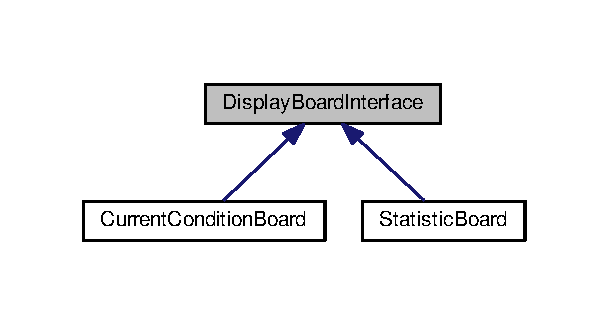
\includegraphics[width=292pt]{classDisplayBoardInterface__inherit__graph}
\end{center}
\end{figure}
\subsection*{Public Member Functions}
\begin{DoxyCompactItemize}
\item 
virtual void \hyperlink{classDisplayBoardInterface_a6a7a21b34415a4b92d290752c75e6f15}{show} ()=0
\end{DoxyCompactItemize}


\subsection{Member Function Documentation}
\index{Display\+Board\+Interface@{Display\+Board\+Interface}!show@{show}}
\index{show@{show}!Display\+Board\+Interface@{Display\+Board\+Interface}}
\subsubsection[{\texorpdfstring{show()=0}{show()=0}}]{\setlength{\rightskip}{0pt plus 5cm}virtual void Display\+Board\+Interface\+::show (
\begin{DoxyParamCaption}
{}
\end{DoxyParamCaption}
)\hspace{0.3cm}{\ttfamily [pure virtual]}}\hypertarget{classDisplayBoardInterface_a6a7a21b34415a4b92d290752c75e6f15}{}\label{classDisplayBoardInterface_a6a7a21b34415a4b92d290752c75e6f15}


Implemented in \hyperlink{classStatisticBoard_a6594f0aac96b441cc8b6c1db1633df55}{Statistic\+Board}, and \hyperlink{classCurrentConditionBoard_a5cd2077415a0e7019c15bc0f28cfb7fe}{Current\+Condition\+Board}.



The documentation for this class was generated from the following file\+:\begin{DoxyCompactItemize}
\item 
\hyperlink{Observer_8cpp}{Observer.\+cpp}\end{DoxyCompactItemize}

\hypertarget{classObserverBoardInterface}{}\section{Observer\+Board\+Interface Class Reference}
\label{classObserverBoardInterface}\index{Observer\+Board\+Interface@{Observer\+Board\+Interface}}


Inheritance diagram for Observer\+Board\+Interface\+:
\nopagebreak
\begin{figure}[H]
\begin{center}
\leavevmode
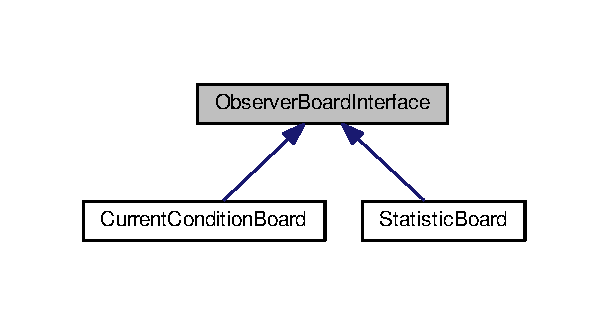
\includegraphics[width=292pt]{classObserverBoardInterface__inherit__graph}
\end{center}
\end{figure}
\subsection*{Public Member Functions}
\begin{DoxyCompactItemize}
\item 
virtual void \hyperlink{classObserverBoardInterface_ae480934d1ef4e49ed6d862ea9f926573}{update} (float a, float b, float c)=0
\end{DoxyCompactItemize}


\subsection{Member Function Documentation}
\index{Observer\+Board\+Interface@{Observer\+Board\+Interface}!update@{update}}
\index{update@{update}!Observer\+Board\+Interface@{Observer\+Board\+Interface}}
\subsubsection[{\texorpdfstring{update(float a, float b, float c)=0}{update(float a, float b, float c)=0}}]{\setlength{\rightskip}{0pt plus 5cm}virtual void Observer\+Board\+Interface\+::update (
\begin{DoxyParamCaption}
\item[{float}]{a, }
\item[{float}]{b, }
\item[{float}]{c}
\end{DoxyParamCaption}
)\hspace{0.3cm}{\ttfamily [pure virtual]}}\hypertarget{classObserverBoardInterface_ae480934d1ef4e49ed6d862ea9f926573}{}\label{classObserverBoardInterface_ae480934d1ef4e49ed6d862ea9f926573}


Implemented in \hyperlink{classStatisticBoard_a9798b65093467a16cd52b2b6f813dbed}{Statistic\+Board}, and \hyperlink{classCurrentConditionBoard_a3d7bea56331de46f30db9e93f8f2c7d3}{Current\+Condition\+Board}.



The documentation for this class was generated from the following file\+:\begin{DoxyCompactItemize}
\item 
\hyperlink{Observer_8cpp}{Observer.\+cpp}\end{DoxyCompactItemize}

\hypertarget{classParaWeatherData}{}\section{Para\+Weather\+Data Class Reference}
\label{classParaWeatherData}\index{Para\+Weather\+Data@{Para\+Weather\+Data}}


Inheritance diagram for Para\+Weather\+Data\+:
\nopagebreak
\begin{figure}[H]
\begin{center}
\leavevmode
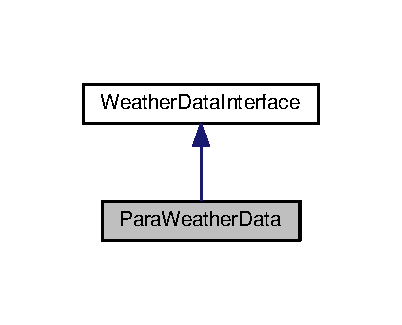
\includegraphics[width=193pt]{classParaWeatherData__inherit__graph}
\end{center}
\end{figure}


Collaboration diagram for Para\+Weather\+Data\+:
\nopagebreak
\begin{figure}[H]
\begin{center}
\leavevmode
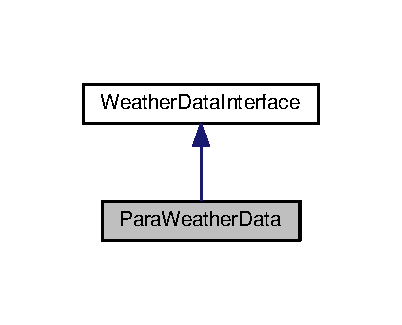
\includegraphics[width=193pt]{classParaWeatherData__coll__graph}
\end{center}
\end{figure}
\subsection*{Public Member Functions}
\begin{DoxyCompactItemize}
\item 
void \hyperlink{classParaWeatherData_a53f58e23b6b2b8b7267fafdd0059bdc6}{Sensor\+Data\+Change} (float a, float b, float c)
\item 
void \hyperlink{classParaWeatherData_a97816831a5acc55f92e1ef3712d1ab37}{register\+Ob} (\hyperlink{classObserverBoardInterface}{Observer\+Board\+Interface} $\ast$ob)
\item 
void \hyperlink{classParaWeatherData_aea026913d5139b73aa5a7e9254d5f251}{remove\+Ob} (\hyperlink{classObserverBoardInterface}{Observer\+Board\+Interface} $\ast$ob)
\end{DoxyCompactItemize}
\subsection*{Protected Member Functions}
\begin{DoxyCompactItemize}
\item 
void \hyperlink{classParaWeatherData_a7bf2ca268e2d6fb932df8012abd08c3d}{notify\+Ob} ()
\end{DoxyCompactItemize}
\subsection*{Private Attributes}
\begin{DoxyCompactItemize}
\item 
float \hyperlink{classParaWeatherData_aeec114146e1053ee8bfc3639705e00c1}{m\+\_\+humidity}
\item 
float \hyperlink{classParaWeatherData_aca752f57b1b7c7a71556cb778b894ff3}{m\+\_\+temperature}
\item 
float \hyperlink{classParaWeatherData_a5e154d46c7b4444aeebb966383eba5b8}{m\+\_\+pressure}
\item 
list$<$ \hyperlink{classObserverBoardInterface}{Observer\+Board\+Interface} $\ast$ $>$ \hyperlink{classParaWeatherData_a876526d1f935d81abc5337051a76334a}{m\+\_\+obs}
\end{DoxyCompactItemize}


\subsection{Member Function Documentation}
\index{Para\+Weather\+Data@{Para\+Weather\+Data}!notify\+Ob@{notify\+Ob}}
\index{notify\+Ob@{notify\+Ob}!Para\+Weather\+Data@{Para\+Weather\+Data}}
\subsubsection[{\texorpdfstring{notify\+Ob()}{notifyOb()}}]{\setlength{\rightskip}{0pt plus 5cm}void Para\+Weather\+Data\+::notify\+Ob (
\begin{DoxyParamCaption}
{}
\end{DoxyParamCaption}
)\hspace{0.3cm}{\ttfamily [inline]}, {\ttfamily [protected]}, {\ttfamily [virtual]}}\hypertarget{classParaWeatherData_a7bf2ca268e2d6fb932df8012abd08c3d}{}\label{classParaWeatherData_a7bf2ca268e2d6fb932df8012abd08c3d}


Implements \hyperlink{classWeatherDataInterface_aef2704c5ad69c82c70b0f8c2f47481c1}{Weather\+Data\+Interface}.


\begin{DoxyCode}
52     \{
53         list<ObserverBoardInterface*>::iterator pos = \hyperlink{classParaWeatherData_a876526d1f935d81abc5337051a76334a}{m\_obs}.begin();
54         \textcolor{keywordflow}{while} (pos != \hyperlink{classParaWeatherData_a876526d1f935d81abc5337051a76334a}{m\_obs}.end())
55         \{
56             ((\hyperlink{classObserverBoardInterface}{ObserverBoardInterface}* )(*pos))->update(
      \hyperlink{classParaWeatherData_aeec114146e1053ee8bfc3639705e00c1}{m\_humidity},\hyperlink{classParaWeatherData_aca752f57b1b7c7a71556cb778b894ff3}{m\_temperature},\hyperlink{classParaWeatherData_a5e154d46c7b4444aeebb966383eba5b8}{m\_pressure});
57             (\textcolor{keyword}{dynamic\_cast<}\hyperlink{classDisplayBoardInterface}{DisplayBoardInterface}*\textcolor{keyword}{>}(*pos))->show();
58             ++pos;
59         \}
60     \}
\end{DoxyCode}
\index{Para\+Weather\+Data@{Para\+Weather\+Data}!register\+Ob@{register\+Ob}}
\index{register\+Ob@{register\+Ob}!Para\+Weather\+Data@{Para\+Weather\+Data}}
\subsubsection[{\texorpdfstring{register\+Ob(\+Observer\+Board\+Interface $\ast$ob)}{registerOb(ObserverBoardInterface *ob)}}]{\setlength{\rightskip}{0pt plus 5cm}void Para\+Weather\+Data\+::register\+Ob (
\begin{DoxyParamCaption}
\item[{{\bf Observer\+Board\+Interface} $\ast$}]{ob}
\end{DoxyParamCaption}
)\hspace{0.3cm}{\ttfamily [inline]}, {\ttfamily [virtual]}}\hypertarget{classParaWeatherData_a97816831a5acc55f92e1ef3712d1ab37}{}\label{classParaWeatherData_a97816831a5acc55f92e1ef3712d1ab37}


Implements \hyperlink{classWeatherDataInterface_ad68a84e0ae106d3ee5289728ce821590}{Weather\+Data\+Interface}.


\begin{DoxyCode}
42     \{
43         \hyperlink{classParaWeatherData_a876526d1f935d81abc5337051a76334a}{m\_obs}.push\_back(ob);
44     \}
\end{DoxyCode}
\index{Para\+Weather\+Data@{Para\+Weather\+Data}!remove\+Ob@{remove\+Ob}}
\index{remove\+Ob@{remove\+Ob}!Para\+Weather\+Data@{Para\+Weather\+Data}}
\subsubsection[{\texorpdfstring{remove\+Ob(\+Observer\+Board\+Interface $\ast$ob)}{removeOb(ObserverBoardInterface *ob)}}]{\setlength{\rightskip}{0pt plus 5cm}void Para\+Weather\+Data\+::remove\+Ob (
\begin{DoxyParamCaption}
\item[{{\bf Observer\+Board\+Interface} $\ast$}]{ob}
\end{DoxyParamCaption}
)\hspace{0.3cm}{\ttfamily [inline]}, {\ttfamily [virtual]}}\hypertarget{classParaWeatherData_aea026913d5139b73aa5a7e9254d5f251}{}\label{classParaWeatherData_aea026913d5139b73aa5a7e9254d5f251}


Implements \hyperlink{classWeatherDataInterface_aa654763e7953baa14c51f0ba67cb947b}{Weather\+Data\+Interface}.


\begin{DoxyCode}
47     \{
48         \hyperlink{classParaWeatherData_a876526d1f935d81abc5337051a76334a}{m\_obs}.remove(ob);
49     \}
\end{DoxyCode}
\index{Para\+Weather\+Data@{Para\+Weather\+Data}!Sensor\+Data\+Change@{Sensor\+Data\+Change}}
\index{Sensor\+Data\+Change@{Sensor\+Data\+Change}!Para\+Weather\+Data@{Para\+Weather\+Data}}
\subsubsection[{\texorpdfstring{Sensor\+Data\+Change(float a, float b, float c)}{SensorDataChange(float a, float b, float c)}}]{\setlength{\rightskip}{0pt plus 5cm}void Para\+Weather\+Data\+::\+Sensor\+Data\+Change (
\begin{DoxyParamCaption}
\item[{float}]{a, }
\item[{float}]{b, }
\item[{float}]{c}
\end{DoxyParamCaption}
)\hspace{0.3cm}{\ttfamily [inline]}}\hypertarget{classParaWeatherData_a53f58e23b6b2b8b7267fafdd0059bdc6}{}\label{classParaWeatherData_a53f58e23b6b2b8b7267fafdd0059bdc6}

\begin{DoxyCode}
34     \{
35         \hyperlink{classParaWeatherData_aeec114146e1053ee8bfc3639705e00c1}{m\_humidity} = a;
36         \hyperlink{classParaWeatherData_aca752f57b1b7c7a71556cb778b894ff3}{m\_temperature} = b;
37         \hyperlink{classParaWeatherData_a5e154d46c7b4444aeebb966383eba5b8}{m\_pressure} = c;
38         \hyperlink{classParaWeatherData_a7bf2ca268e2d6fb932df8012abd08c3d}{notifyOb}();
39     \}
\end{DoxyCode}


\subsection{Member Data Documentation}
\index{Para\+Weather\+Data@{Para\+Weather\+Data}!m\+\_\+humidity@{m\+\_\+humidity}}
\index{m\+\_\+humidity@{m\+\_\+humidity}!Para\+Weather\+Data@{Para\+Weather\+Data}}
\subsubsection[{\texorpdfstring{m\+\_\+humidity}{m_humidity}}]{\setlength{\rightskip}{0pt plus 5cm}float Para\+Weather\+Data\+::m\+\_\+humidity\hspace{0.3cm}{\ttfamily [private]}}\hypertarget{classParaWeatherData_aeec114146e1053ee8bfc3639705e00c1}{}\label{classParaWeatherData_aeec114146e1053ee8bfc3639705e00c1}
\index{Para\+Weather\+Data@{Para\+Weather\+Data}!m\+\_\+obs@{m\+\_\+obs}}
\index{m\+\_\+obs@{m\+\_\+obs}!Para\+Weather\+Data@{Para\+Weather\+Data}}
\subsubsection[{\texorpdfstring{m\+\_\+obs}{m_obs}}]{\setlength{\rightskip}{0pt plus 5cm}list$<${\bf Observer\+Board\+Interface}$\ast$ $>$ Para\+Weather\+Data\+::m\+\_\+obs\hspace{0.3cm}{\ttfamily [private]}}\hypertarget{classParaWeatherData_a876526d1f935d81abc5337051a76334a}{}\label{classParaWeatherData_a876526d1f935d81abc5337051a76334a}
\index{Para\+Weather\+Data@{Para\+Weather\+Data}!m\+\_\+pressure@{m\+\_\+pressure}}
\index{m\+\_\+pressure@{m\+\_\+pressure}!Para\+Weather\+Data@{Para\+Weather\+Data}}
\subsubsection[{\texorpdfstring{m\+\_\+pressure}{m_pressure}}]{\setlength{\rightskip}{0pt plus 5cm}float Para\+Weather\+Data\+::m\+\_\+pressure\hspace{0.3cm}{\ttfamily [private]}}\hypertarget{classParaWeatherData_a5e154d46c7b4444aeebb966383eba5b8}{}\label{classParaWeatherData_a5e154d46c7b4444aeebb966383eba5b8}
\index{Para\+Weather\+Data@{Para\+Weather\+Data}!m\+\_\+temperature@{m\+\_\+temperature}}
\index{m\+\_\+temperature@{m\+\_\+temperature}!Para\+Weather\+Data@{Para\+Weather\+Data}}
\subsubsection[{\texorpdfstring{m\+\_\+temperature}{m_temperature}}]{\setlength{\rightskip}{0pt plus 5cm}float Para\+Weather\+Data\+::m\+\_\+temperature\hspace{0.3cm}{\ttfamily [private]}}\hypertarget{classParaWeatherData_aca752f57b1b7c7a71556cb778b894ff3}{}\label{classParaWeatherData_aca752f57b1b7c7a71556cb778b894ff3}


The documentation for this class was generated from the following file\+:\begin{DoxyCompactItemize}
\item 
\hyperlink{Observer_8cpp}{Observer.\+cpp}\end{DoxyCompactItemize}

\hypertarget{classStatisticBoard}{}\section{Statistic\+Board Class Reference}
\label{classStatisticBoard}\index{Statistic\+Board@{Statistic\+Board}}


Inheritance diagram for Statistic\+Board\+:
\nopagebreak
\begin{figure}[H]
\begin{center}
\leavevmode
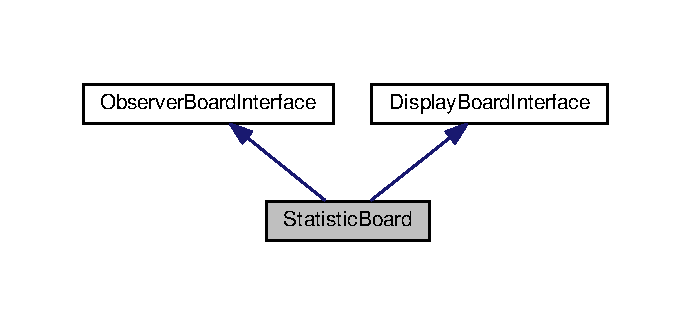
\includegraphics[width=332pt]{classStatisticBoard__inherit__graph}
\end{center}
\end{figure}


Collaboration diagram for Statistic\+Board\+:
\nopagebreak
\begin{figure}[H]
\begin{center}
\leavevmode
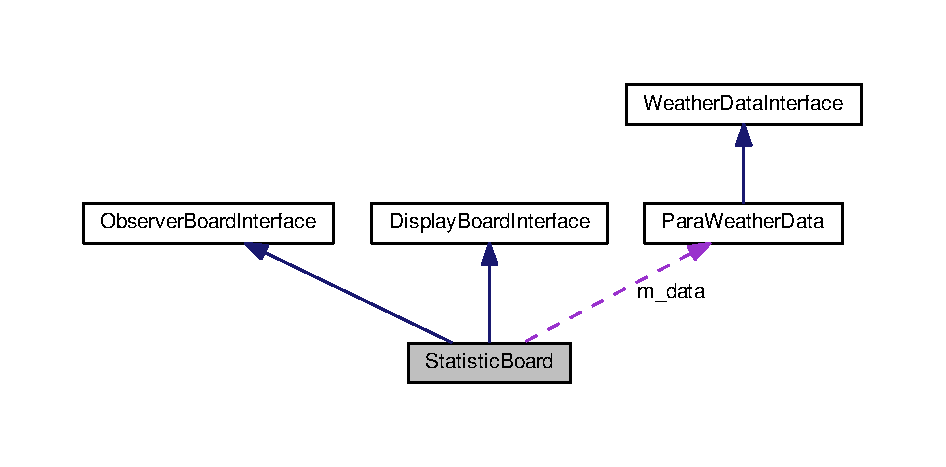
\includegraphics[width=350pt]{classStatisticBoard__coll__graph}
\end{center}
\end{figure}
\subsection*{Public Member Functions}
\begin{DoxyCompactItemize}
\item 
\hyperlink{classStatisticBoard_aec1eb00966e7d219ac20a97f0810bc93}{Statistic\+Board} (\hyperlink{classParaWeatherData}{Para\+Weather\+Data} \&a)
\item 
void \hyperlink{classStatisticBoard_a6594f0aac96b441cc8b6c1db1633df55}{show} ()
\item 
void \hyperlink{classStatisticBoard_a9798b65093467a16cd52b2b6f813dbed}{update} (float h, float t, float p)
\end{DoxyCompactItemize}
\subsection*{Private Attributes}
\begin{DoxyCompactItemize}
\item 
float \hyperlink{classStatisticBoard_ae44658877f1ef0413ab0212671de455a}{m\+\_\+maxt}
\item 
float \hyperlink{classStatisticBoard_a7d8f109c876c413a035c356e19f59b6f}{m\+\_\+mint}
\item 
float \hyperlink{classStatisticBoard_a942352228021cc8ab83848ffd2c2e92e}{m\+\_\+avet}
\item 
int \hyperlink{classStatisticBoard_ad08df42fbc4bfd6a738d70c7bb275d27}{m\+\_\+count}
\item 
\hyperlink{classParaWeatherData}{Para\+Weather\+Data} \& \hyperlink{classStatisticBoard_a53d2b170ec3d9127fe13bd9d3cc751d7}{m\+\_\+data}
\end{DoxyCompactItemize}


\subsection{Constructor \& Destructor Documentation}
\index{Statistic\+Board@{Statistic\+Board}!Statistic\+Board@{Statistic\+Board}}
\index{Statistic\+Board@{Statistic\+Board}!Statistic\+Board@{Statistic\+Board}}
\subsubsection[{\texorpdfstring{Statistic\+Board(\+Para\+Weather\+Data \&a)}{StatisticBoard(ParaWeatherData &a)}}]{\setlength{\rightskip}{0pt plus 5cm}Statistic\+Board\+::\+Statistic\+Board (
\begin{DoxyParamCaption}
\item[{{\bf Para\+Weather\+Data} \&}]{a}
\end{DoxyParamCaption}
)\hspace{0.3cm}{\ttfamily [inline]}}\hypertarget{classStatisticBoard_aec1eb00966e7d219ac20a97f0810bc93}{}\label{classStatisticBoard_aec1eb00966e7d219ac20a97f0810bc93}

\begin{DoxyCode}
104                                       :\hyperlink{classStatisticBoard_ae44658877f1ef0413ab0212671de455a}{m\_maxt}(-1000),\hyperlink{classStatisticBoard_a7d8f109c876c413a035c356e19f59b6f}{m\_mint}(1000),
      \hyperlink{classStatisticBoard_a942352228021cc8ab83848ffd2c2e92e}{m\_avet}(0),\hyperlink{classStatisticBoard_ad08df42fbc4bfd6a738d70c7bb275d27}{m\_count}(0),\hyperlink{classStatisticBoard_a53d2b170ec3d9127fe13bd9d3cc751d7}{m\_data}(a)
105     \{
106         \hyperlink{classStatisticBoard_a53d2b170ec3d9127fe13bd9d3cc751d7}{m\_data}.\hyperlink{classParaWeatherData_a97816831a5acc55f92e1ef3712d1ab37}{registerOb}(\textcolor{keyword}{this});
107     \}
\end{DoxyCode}


\subsection{Member Function Documentation}
\index{Statistic\+Board@{Statistic\+Board}!show@{show}}
\index{show@{show}!Statistic\+Board@{Statistic\+Board}}
\subsubsection[{\texorpdfstring{show()}{show()}}]{\setlength{\rightskip}{0pt plus 5cm}void Statistic\+Board\+::show (
\begin{DoxyParamCaption}
{}
\end{DoxyParamCaption}
)\hspace{0.3cm}{\ttfamily [inline]}, {\ttfamily [virtual]}}\hypertarget{classStatisticBoard_a6594f0aac96b441cc8b6c1db1633df55}{}\label{classStatisticBoard_a6594f0aac96b441cc8b6c1db1633df55}


Implements \hyperlink{classDisplayBoardInterface_a6a7a21b34415a4b92d290752c75e6f15}{Display\+Board\+Interface}.


\begin{DoxyCode}
110     \{
111         cout<<\textcolor{stringliteral}{"\_\_\_\_\_\_\_\_StatisticBoard\_\_\_\_\_\_\_\_\_"}<<endl;
112         cout<<\textcolor{stringliteral}{"lowest  temperature: "}<<\hyperlink{classStatisticBoard_a7d8f109c876c413a035c356e19f59b6f}{m\_mint}<<endl;
113         cout<<\textcolor{stringliteral}{"highest temperature: "}<<\hyperlink{classStatisticBoard_ae44658877f1ef0413ab0212671de455a}{m\_maxt}<<endl;
114         cout<<\textcolor{stringliteral}{"average temperature: "}<<\hyperlink{classStatisticBoard_a942352228021cc8ab83848ffd2c2e92e}{m\_avet}<<endl;
115         cout<<\textcolor{stringliteral}{"\_\_\_\_\_\_\_\_\_\_\_\_\_\_\_\_\_\_\_\_\_\_\_\_\_\_\_\_\_\_\_"}<<endl;
116     \}
\end{DoxyCode}
\index{Statistic\+Board@{Statistic\+Board}!update@{update}}
\index{update@{update}!Statistic\+Board@{Statistic\+Board}}
\subsubsection[{\texorpdfstring{update(float h, float t, float p)}{update(float h, float t, float p)}}]{\setlength{\rightskip}{0pt plus 5cm}void Statistic\+Board\+::update (
\begin{DoxyParamCaption}
\item[{float}]{h, }
\item[{float}]{t, }
\item[{float}]{p}
\end{DoxyParamCaption}
)\hspace{0.3cm}{\ttfamily [inline]}, {\ttfamily [virtual]}}\hypertarget{classStatisticBoard_a9798b65093467a16cd52b2b6f813dbed}{}\label{classStatisticBoard_a9798b65093467a16cd52b2b6f813dbed}


Implements \hyperlink{classObserverBoardInterface_ae480934d1ef4e49ed6d862ea9f926573}{Observer\+Board\+Interface}.


\begin{DoxyCode}
119     \{
120         ++\hyperlink{classStatisticBoard_ad08df42fbc4bfd6a738d70c7bb275d27}{m\_count};
121         \textcolor{keywordflow}{if} (t>\hyperlink{classStatisticBoard_ae44658877f1ef0413ab0212671de455a}{m\_maxt})
122         \{
123             \hyperlink{classStatisticBoard_ae44658877f1ef0413ab0212671de455a}{m\_maxt} = t;
124         \}
125         \textcolor{keywordflow}{if} (t<\hyperlink{classStatisticBoard_a7d8f109c876c413a035c356e19f59b6f}{m\_mint})
126         \{
127             \hyperlink{classStatisticBoard_a7d8f109c876c413a035c356e19f59b6f}{m\_mint} = t;
128         \}
129         \hyperlink{classStatisticBoard_a942352228021cc8ab83848ffd2c2e92e}{m\_avet} = (\hyperlink{classStatisticBoard_a942352228021cc8ab83848ffd2c2e92e}{m\_avet} * (\hyperlink{classStatisticBoard_ad08df42fbc4bfd6a738d70c7bb275d27}{m\_count}-1) + t)/\hyperlink{classStatisticBoard_ad08df42fbc4bfd6a738d70c7bb275d27}{m\_count};
130     \}
\end{DoxyCode}


\subsection{Member Data Documentation}
\index{Statistic\+Board@{Statistic\+Board}!m\+\_\+avet@{m\+\_\+avet}}
\index{m\+\_\+avet@{m\+\_\+avet}!Statistic\+Board@{Statistic\+Board}}
\subsubsection[{\texorpdfstring{m\+\_\+avet}{m_avet}}]{\setlength{\rightskip}{0pt plus 5cm}float Statistic\+Board\+::m\+\_\+avet\hspace{0.3cm}{\ttfamily [private]}}\hypertarget{classStatisticBoard_a942352228021cc8ab83848ffd2c2e92e}{}\label{classStatisticBoard_a942352228021cc8ab83848ffd2c2e92e}
\index{Statistic\+Board@{Statistic\+Board}!m\+\_\+count@{m\+\_\+count}}
\index{m\+\_\+count@{m\+\_\+count}!Statistic\+Board@{Statistic\+Board}}
\subsubsection[{\texorpdfstring{m\+\_\+count}{m_count}}]{\setlength{\rightskip}{0pt plus 5cm}int Statistic\+Board\+::m\+\_\+count\hspace{0.3cm}{\ttfamily [private]}}\hypertarget{classStatisticBoard_ad08df42fbc4bfd6a738d70c7bb275d27}{}\label{classStatisticBoard_ad08df42fbc4bfd6a738d70c7bb275d27}
\index{Statistic\+Board@{Statistic\+Board}!m\+\_\+data@{m\+\_\+data}}
\index{m\+\_\+data@{m\+\_\+data}!Statistic\+Board@{Statistic\+Board}}
\subsubsection[{\texorpdfstring{m\+\_\+data}{m_data}}]{\setlength{\rightskip}{0pt plus 5cm}{\bf Para\+Weather\+Data}\& Statistic\+Board\+::m\+\_\+data\hspace{0.3cm}{\ttfamily [private]}}\hypertarget{classStatisticBoard_a53d2b170ec3d9127fe13bd9d3cc751d7}{}\label{classStatisticBoard_a53d2b170ec3d9127fe13bd9d3cc751d7}
\index{Statistic\+Board@{Statistic\+Board}!m\+\_\+maxt@{m\+\_\+maxt}}
\index{m\+\_\+maxt@{m\+\_\+maxt}!Statistic\+Board@{Statistic\+Board}}
\subsubsection[{\texorpdfstring{m\+\_\+maxt}{m_maxt}}]{\setlength{\rightskip}{0pt plus 5cm}float Statistic\+Board\+::m\+\_\+maxt\hspace{0.3cm}{\ttfamily [private]}}\hypertarget{classStatisticBoard_ae44658877f1ef0413ab0212671de455a}{}\label{classStatisticBoard_ae44658877f1ef0413ab0212671de455a}
\index{Statistic\+Board@{Statistic\+Board}!m\+\_\+mint@{m\+\_\+mint}}
\index{m\+\_\+mint@{m\+\_\+mint}!Statistic\+Board@{Statistic\+Board}}
\subsubsection[{\texorpdfstring{m\+\_\+mint}{m_mint}}]{\setlength{\rightskip}{0pt plus 5cm}float Statistic\+Board\+::m\+\_\+mint\hspace{0.3cm}{\ttfamily [private]}}\hypertarget{classStatisticBoard_a7d8f109c876c413a035c356e19f59b6f}{}\label{classStatisticBoard_a7d8f109c876c413a035c356e19f59b6f}


The documentation for this class was generated from the following file\+:\begin{DoxyCompactItemize}
\item 
\hyperlink{Observer_8cpp}{Observer.\+cpp}\end{DoxyCompactItemize}

\hypertarget{classWeatherDataInterface}{}\section{Weather\+Data\+Interface Class Reference}
\label{classWeatherDataInterface}\index{Weather\+Data\+Interface@{Weather\+Data\+Interface}}


Inheritance diagram for Weather\+Data\+Interface\+:
\nopagebreak
\begin{figure}[H]
\begin{center}
\leavevmode
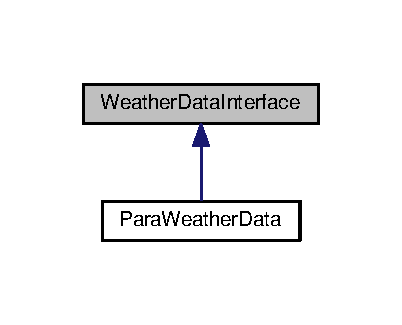
\includegraphics[width=193pt]{classWeatherDataInterface__inherit__graph}
\end{center}
\end{figure}
\subsection*{Public Member Functions}
\begin{DoxyCompactItemize}
\item 
virtual void \hyperlink{classWeatherDataInterface_ad68a84e0ae106d3ee5289728ce821590}{register\+Ob} (\hyperlink{classObserverBoardInterface}{Observer\+Board\+Interface} $\ast$ob)=0
\item 
virtual void \hyperlink{classWeatherDataInterface_aa654763e7953baa14c51f0ba67cb947b}{remove\+Ob} (\hyperlink{classObserverBoardInterface}{Observer\+Board\+Interface} $\ast$ob)=0
\item 
virtual void \hyperlink{classWeatherDataInterface_aef2704c5ad69c82c70b0f8c2f47481c1}{notify\+Ob} ()=0
\end{DoxyCompactItemize}


\subsection{Member Function Documentation}
\index{Weather\+Data\+Interface@{Weather\+Data\+Interface}!notify\+Ob@{notify\+Ob}}
\index{notify\+Ob@{notify\+Ob}!Weather\+Data\+Interface@{Weather\+Data\+Interface}}
\subsubsection[{\texorpdfstring{notify\+Ob()=0}{notifyOb()=0}}]{\setlength{\rightskip}{0pt plus 5cm}virtual void Weather\+Data\+Interface\+::notify\+Ob (
\begin{DoxyParamCaption}
{}
\end{DoxyParamCaption}
)\hspace{0.3cm}{\ttfamily [pure virtual]}}\hypertarget{classWeatherDataInterface_aef2704c5ad69c82c70b0f8c2f47481c1}{}\label{classWeatherDataInterface_aef2704c5ad69c82c70b0f8c2f47481c1}


Implemented in \hyperlink{classParaWeatherData_a7bf2ca268e2d6fb932df8012abd08c3d}{Para\+Weather\+Data}.

\index{Weather\+Data\+Interface@{Weather\+Data\+Interface}!register\+Ob@{register\+Ob}}
\index{register\+Ob@{register\+Ob}!Weather\+Data\+Interface@{Weather\+Data\+Interface}}
\subsubsection[{\texorpdfstring{register\+Ob(\+Observer\+Board\+Interface $\ast$ob)=0}{registerOb(ObserverBoardInterface *ob)=0}}]{\setlength{\rightskip}{0pt plus 5cm}virtual void Weather\+Data\+Interface\+::register\+Ob (
\begin{DoxyParamCaption}
\item[{{\bf Observer\+Board\+Interface} $\ast$}]{ob}
\end{DoxyParamCaption}
)\hspace{0.3cm}{\ttfamily [pure virtual]}}\hypertarget{classWeatherDataInterface_ad68a84e0ae106d3ee5289728ce821590}{}\label{classWeatherDataInterface_ad68a84e0ae106d3ee5289728ce821590}


Implemented in \hyperlink{classParaWeatherData_a97816831a5acc55f92e1ef3712d1ab37}{Para\+Weather\+Data}.

\index{Weather\+Data\+Interface@{Weather\+Data\+Interface}!remove\+Ob@{remove\+Ob}}
\index{remove\+Ob@{remove\+Ob}!Weather\+Data\+Interface@{Weather\+Data\+Interface}}
\subsubsection[{\texorpdfstring{remove\+Ob(\+Observer\+Board\+Interface $\ast$ob)=0}{removeOb(ObserverBoardInterface *ob)=0}}]{\setlength{\rightskip}{0pt plus 5cm}virtual void Weather\+Data\+Interface\+::remove\+Ob (
\begin{DoxyParamCaption}
\item[{{\bf Observer\+Board\+Interface} $\ast$}]{ob}
\end{DoxyParamCaption}
)\hspace{0.3cm}{\ttfamily [pure virtual]}}\hypertarget{classWeatherDataInterface_aa654763e7953baa14c51f0ba67cb947b}{}\label{classWeatherDataInterface_aa654763e7953baa14c51f0ba67cb947b}


Implemented in \hyperlink{classParaWeatherData_aea026913d5139b73aa5a7e9254d5f251}{Para\+Weather\+Data}.



The documentation for this class was generated from the following file\+:\begin{DoxyCompactItemize}
\item 
\hyperlink{Observer_8cpp}{Observer.\+cpp}\end{DoxyCompactItemize}

\chapter{File Documentation}
\hypertarget{Observer_8cpp}{}\section{Observer.\+cpp File Reference}
\label{Observer_8cpp}\index{Observer.\+cpp@{Observer.\+cpp}}
{\ttfamily \#include $<$list$>$}\\*
{\ttfamily \#include $<$algorithm$>$}\\*
{\ttfamily \#include $<$iostream$>$}\\*
Include dependency graph for Observer.\+cpp\+:
\nopagebreak
\begin{figure}[H]
\begin{center}
\leavevmode
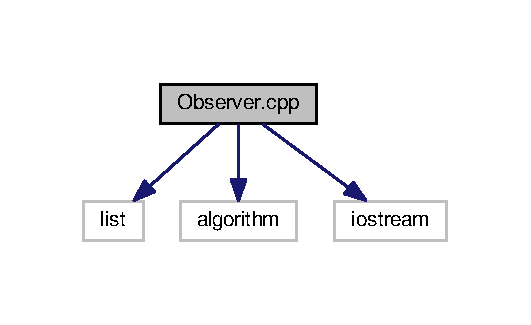
\includegraphics[width=255pt]{Observer_8cpp__incl}
\end{center}
\end{figure}
\subsection*{Classes}
\begin{DoxyCompactItemize}
\item 
class \hyperlink{classObserverBoardInterface}{Observer\+Board\+Interface}
\item 
class \hyperlink{classDisplayBoardInterface}{Display\+Board\+Interface}
\item 
class \hyperlink{classWeatherDataInterface}{Weather\+Data\+Interface}
\item 
class \hyperlink{classParaWeatherData}{Para\+Weather\+Data}
\item 
class \hyperlink{classCurrentConditionBoard}{Current\+Condition\+Board}
\item 
class \hyperlink{classStatisticBoard}{Statistic\+Board}
\end{DoxyCompactItemize}
\subsection*{Functions}
\begin{DoxyCompactItemize}
\item 
int \hyperlink{Observer_8cpp_a0ddf1224851353fc92bfbff6f499fa97}{main} (int argc, char $\ast$argv\mbox{[}$\,$\mbox{]})
\end{DoxyCompactItemize}


\subsection{Function Documentation}
\index{Observer.\+cpp@{Observer.\+cpp}!main@{main}}
\index{main@{main}!Observer.\+cpp@{Observer.\+cpp}}
\subsubsection[{\texorpdfstring{main(int argc, char $\ast$argv[])}{main(int argc, char *argv[])}}]{\setlength{\rightskip}{0pt plus 5cm}int main (
\begin{DoxyParamCaption}
\item[{int}]{argc, }
\item[{char $\ast$}]{argv\mbox{[}$\,$\mbox{]}}
\end{DoxyParamCaption}
)}\hypertarget{Observer_8cpp_a0ddf1224851353fc92bfbff6f499fa97}{}\label{Observer_8cpp_a0ddf1224851353fc92bfbff6f499fa97}

\begin{DoxyCode}
142 \{
143    
144     \hyperlink{classParaWeatherData}{ParaWeatherData} * wdata = \textcolor{keyword}{new} \hyperlink{classParaWeatherData}{ParaWeatherData};
145     \hyperlink{classCurrentConditionBoard}{CurrentConditionBoard}* currentB = \textcolor{keyword}{new} 
      \hyperlink{classCurrentConditionBoard}{CurrentConditionBoard}(*wdata);
146     \hyperlink{classStatisticBoard}{StatisticBoard}* statisticB = \textcolor{keyword}{new} \hyperlink{classStatisticBoard}{StatisticBoard}(*wdata);
147 
148     wdata->\hyperlink{classParaWeatherData_a53f58e23b6b2b8b7267fafdd0059bdc6}{SensorDataChange}(10.2, 28.2, 1001);
149     wdata->\hyperlink{classParaWeatherData_a53f58e23b6b2b8b7267fafdd0059bdc6}{SensorDataChange}(12, 30.12, 1003);
150     wdata->\hyperlink{classParaWeatherData_a53f58e23b6b2b8b7267fafdd0059bdc6}{SensorDataChange}(10.2, 26, 806);
151     wdata->\hyperlink{classParaWeatherData_a53f58e23b6b2b8b7267fafdd0059bdc6}{SensorDataChange}(10.3, 35.9, 900);
152 
153     wdata->\hyperlink{classParaWeatherData_aea026913d5139b73aa5a7e9254d5f251}{removeOb}(currentB);
154 
155     wdata->\hyperlink{classParaWeatherData_a53f58e23b6b2b8b7267fafdd0059bdc6}{SensorDataChange}(100, 40, 1900);  
156     
157     \textcolor{keyword}{delete} statisticB;
158     \textcolor{keyword}{delete} currentB;
159     \textcolor{keyword}{delete} wdata;
160 
161     \textcolor{keywordflow}{return} 0;
162 \}\end{DoxyCode}


Here is the call graph for this function\+:
\nopagebreak
\begin{figure}[H]
\begin{center}
\leavevmode
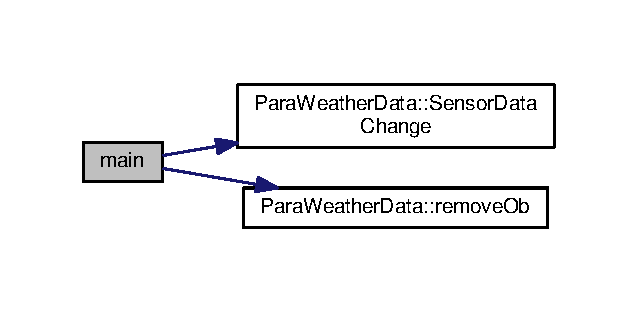
\includegraphics[width=306pt]{Observer_8cpp_a0ddf1224851353fc92bfbff6f499fa97_cgraph}
\end{center}
\end{figure}



%--- End generated contents ---

% Index
\backmatter
\newpage
\phantomsection
\clearemptydoublepage
\addcontentsline{toc}{chapter}{Index}
\printindex

\end{document}
